\chapter{Twin Study}
\label{ch:twin}

\section{Introduction}
The very first blockchain system, that is Bitcoin~\cite{nakamoto2019bitcoin}, is a decentralized ledger for
recording cryptocurrency's transactions. The ledger consists of multiple blocks chained together with cryptographic
hash pointers, each block containing multiple transactions. This chain of blocks is distributed    
across a network of nodes, some of which behave in a Byzantine (or malicious) manner~\cite{Lamport_BFT}. The network runs a
consensus protocol, namely \textit{proof-of-work} (PoW), to keep the ledger consistent among the nodes.  

Bitcoin is the first digital currency (or cryptocurrency) system that
operates in a Byzantine \cite{Lamport_BFT} peer-to-peer (P2P) environment, without relying on a common trusted
third party.
But it can execute only simple transactions that move some coins from one address (or user) to another.
Recent blockchains such as Ethereum~\cite{wood2014ethereum} and Hyperledger
Fabric~\cite{androulaki2018hyperledger} support general-purpose transactions. The key enabler is the {\em
smart contract} --- a user-defined computation executed by all nodes in the blockchain. 
With smart contracts, blockchains can execute transactional workloads which have so far been handled almost
exclusively by 
databases.  In other words, blockchains have evolved into transactional management systems, and therefore are
comparable to distributed databases. Their advantages over the latter include data transparency and security
against Byzantine failures. 
In fact, many companies and government agencies are exploring blockchains to replace, or to complement, their
enterprise-grade databases~\cite{mougayar2016business,morabito2017business,crosby2016blockchain}.

The parallel between blockchains and distributed databases has not gone unnoticed. Existing works show that
there are little similarities between the two. Blockchains are suitable when the applications are running in
untrusted, hostile environments, whereas databases are
suitable when performance is more important than
security~\cite{crosby2016blockchain, wust2018you,chowdhury2018blockchain,yaga2018blockchain}. Their distinction is further compounded
by the significant gap in performance~\cite{dinh2017blockbench}, for instance Bitcoin processes around
$10$ transactions per second~\cite{bitcoin_tps} while etcd --- a state-of-the-art distributed NoSQL database
--- processes over $50,000$ operations per second~\cite{etcd_perf}.

On the other hand, we notice the trend of design fusion between databases and blockchains. Design principles and techniques that are traditionally used by databases are being adopted by blockchains. For example, concurrency control techniques attributed to databases are used to increase the performance of blockchains~\cite{sharma2019blurring, ruan2020transactional, dickerson2017adding}. Moreover, sharding has been used to scale out permissioned blockchains~\cite{dang2019towards}. At the same time, the security features of blockchains are used in hybrid blockchain-database systems to provide verifiable data~\cite{el2019blockchaindb, veritas, peng2020falcondb}. 

One limitation of the existing works that compare blockchains and databases is that they only focus on
application-level, observable and measurable properties, such as throughput and security. In particular, they
show how the two types of systems differ without identifying the root cause. For example, 
BLOCKBENCH~\cite{dinh2017blockbench} compares three permissioned blockchains, namely Hyperledger Fabric, Ethereum
and Parity, with H-Store under two popular data processing workloads. It shows a large gap in performance, but provides no further analysis of the gap. As a consequence, the reported difference does not
generalize to other workloads other than the two used in the experiments. For instance, under high contention
workloads, the performance difference may shrink drastically, or may even reverse.   

We aim to provide a comprehensive dichotomy of blockchains and databases. Our approach is to position  
them within the same design space --- that is, the design space of general transactional systems. We propose a
taxonomy consisting of four design dimensions and discuss how the two types of systems make different design choices in
each dimension. The first dimension is replication, which determines what data is replicated to what nodes,
and the mechanism needed to keep the replicas consistent. The second is concurrency, which determines the tradeoffs between performance and correctness when executing concurrent transactions. The third is storage, which
determines the data models and access methods. The final dimension is sharding, which determines how data is
partitioned, and the mechanism for atomicity of cross-shard transactions.  

Under our taxonomy, existing works such as~\cite{dinh2017blockbench} are incomplete: they only cover extreme
points in the design space. In contrast, our work is comprehensive, as it covers many other
points in the space. Our taxonomy illustrates the inherent similarities between blockchains and
databases, and provides a principled framework for exploring new designs that fuse blockchains and
databases~\cite{BlockchainMeetsDatabase,peng2020falcondb,veritas,el2019blockchaindb,mcconaghy2016bigchaindb,schuhknecht2019chainifydb}. 
We observe that both systems address the same set of
problems in distributed settings, including consistency, failure and data access, but they make different
design choices driven by the high-level goals: security for blockchains and performance for databases.  Given
the taxonomy, we conduct experiments to evaluate the effect of different design choices, thereby giving
insights into the factors that contribute to their performance gap.  

In summary, we make the following contributions:
\begin{itemize}
  \item We compare blockchains and distributed databases as two different types of distributed, transactional systems.  We propose a new taxonomy that characterizes both system categories and their hybrids along four design dimensions: replication, concurrency, storage, and sharding.

  \item We use our taxonomy to analyze the security and performance of emerging hybrid blockchain-database systems. 
  
  \item We conduct a comprehensive performance study of five popular systems, including  two permissioned blockchains, namely Hyperledger Fabric and Quorum, and three database systems, namely CockroachDB, TiDB, and etcd. The results demonstrate the impact of different design choices on the overall performance. 

\end{itemize}

\Cref{twin:sec:background} provides relevant background, followed by a qualitative comparisons on the above
four dimensions in \Cref{twin:sec:anatomy}. \Cref{twin:sec:setup} and \Cref{twin:sec:result} discuss the experimental setup and
results, respectively. 

\section{Background}
\label{twin:sec:background}
In this section, we discuss relevant background on blockchains and distributed databases.
Figure~\ref{diagram:twin:spectrum} shows a high-level comparison of these systems.

\begin{figure}
    \centering
    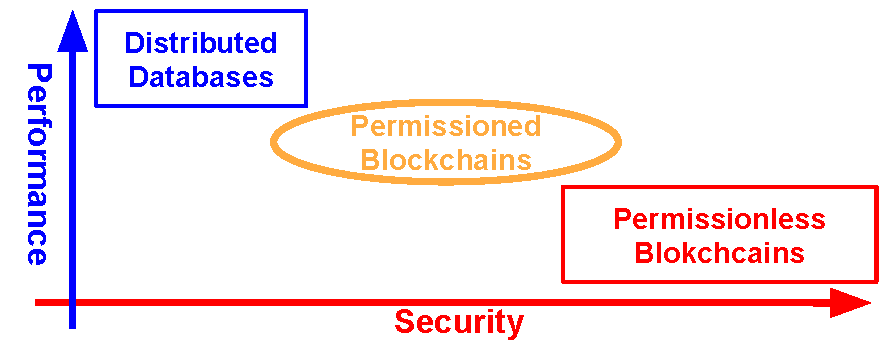
\includegraphics[width=0.9\textwidth]{diagram/twin/spectrum.pdf}
    \caption{Blockchains vs. distributed databases in the security-performance coordinate.}
    \label{diagram:twin:spectrum} 
\end{figure}

\subsection{Blockchain}
From a data structure perspective, a blockchain is a list of blocks linked by cryptographic hash pointers. These blocks contain cryptocurrency transactions~\cite{nakamoto2019bitcoin}. By this definition, the blockchain is a tamper-evident ledger for recording transactions. With smart contracts, transactions are in the form of contract deployment and invocation.
From a systems perspective, a blockchain is a distributed system consisting of multiple nodes, some of which are malicious. These nodes maintain a consistent ledger by using a Byzantine fault-tolerant (BFT) consensus protocol, such as PoW or PBFT~\cite{castro1999practical}.

In the earlier designs, a blockchain transaction is restricted to cryptocurrency and the states are modeled
as Unspent Transaction Outputs (UTXO).  For example, Bitcoin~\cite{nakamoto2019bitcoin} and other similar
altcoins use the UTXO model.  Starting with Ethereum~\cite{wood2014ethereum}, blockchains support \textit{smart
contracts} which allow users to encode and execute arbitrary Turing-complete computations on the ledger. The ledger states are modelled as accounts instead of UTXO. 
Other systems supporting smart contracts include Quorum, Parity and Hyperledger Fabric~\cite{androulaki2018hyperledger}.  In these systems, a transaction on the ledger takes the form of a contract invocation, which modifies the ledger based on order determined by the consensus protocol. A read-only transaction can be carried out by any node, without undergoing the consensus and being included in the ledger. We only consider blockchains that support smart contracts in this paper, because earlier blockchains (without smart contracts) cannot support database transaction workloads and thus cannot be compared with distributed databases.

\textbf{Permissionless vs. Permissioned.} Blockchains can be broadly divided into two categories: permissionless (or public), and permissioned (or
private). In the former, for example in Bitcoin and Ethereum, any node and user can join the system in a pseudonymous manner. In the latter, for example in Fabric and Quorum, the node and user must be authorized to join the system. With strong membership control and action regulation, permissioned blockchains are more suitable for enterprise applications and are particularly used in the financial sector.
Figure~\ref{diagram:twin:spectrum} shows the security-performance tradeoffs in blockchains. It highlights how permissionless
blockchains can achieve stronger security because they make no identity assumption. In contrast, permissioned
blockchains have weaker security because of the identity assumption, but can achieve higher performance
because they can employ consensus protocols with higher efficiency. A more detailed discussion of permissionless versus permissioned blockchain designs can be found
in~\cite{dinh2018untangling,dinh2017blockbench}.


\subsection{Distributed Databases}

Unlike blockchains, database systems have been around for decades.  Relational databases, which  
support easy-to-use SQL language and intuitive ACID transaction semantics, remained mainstream throughout the years. The recent demand of big data processing and the fact that Moore's law is reaching its limit are major factors
behind the trend of scale-out database designs. Nowadays, both data and computation are distributed over multiple nodes
in order to achieve high availability and scalability. Principles and techniques in designing and scaling distributed databases are described in detail in~\cite{ozsu2011principles}. 
Basically, there are two distinctive movements, namely NoSQL and NewSQL, under this new design direction.


\textbf{NoSQL vs. NewSQL.}
For scalability, many distributed databases abandon the complex relational model and
the strong ACID semantics. 
These systems are referred to as {\em NoSQL}. They support more flexible data models and weaker consistency. 
% They adopt the BASE principle for their transaction semantics. 
In the sense of CAP theorem~\cite{gilbert2012perspectives}, these NoSQL systems compromise consistency for the sake of availability. 
A variety of their supported data models may include key-value store (e.g, Redis~\cite{carlson2013redis}, etcd~\cite{web:etcd}), 
document store (e.g, CouchDB~\cite{anderson2010couchdb}), graph store (e.g, Neo4J~\cite{vukotic2014neo4j}), column-oriented (e.g, Cassandra~\cite{lakshman2010cassandra}) and so on. 
The most lenient consistency model is eventual consistency which makes no guarantees about the order
of read and write operations. 
Between eventual and strong consistency, researchers explore a variety of other abstractions, such as sequential, causal and PRAM consistency. They standardize on the allowable operation behavior for the ease of reasoning. 
Most NoSQL databases offer configurable options, where users can tradeoff between performance and consistency.

The surge of NoSQL systems, however, does not obscure the cost in usability and
the increase in application complexity.  A new class of distributed database systems, called {\em NewSQL}, aim to restore the relational model and ACID semantics without sacrificing much scalability.  
NewSQL has drawn attention since 

Google introduced Spanner~\cite{corbett2013spanner}, the first NewSQL system. It was followed by a few database vendors, such as CockroachDB~\cite{taft2020cockroachdb} and TiDB~\cite{huang13tidb}. In this paper, we consider both NoSQL and NewSQL systems.

\section{Taxonomy}
\label{twin:sec:anatomy}
In this section, we present a distributed system taxonomy that illustrates the important design choices made
by blockchains and distributed databases. We highlight how the differences are driven by the fact that these
systems aim to achieve different goals: security for blockchains, and performance for databases.  
Table~\ref{twin:tab:taxonomy} compares the design choices of distributed databases and blockchains under each dimension in our taxonomy. 

\begin{table}
	\centering
	\caption{Design choices in blockchains and distributed databases}
    \label{twin:tab:taxonomy}
	% \toprule
	
\begin{tabular}{l|p{0.38\textwidth}p{0.35\textwidth}}
                     & \textbf{Blockchains}                                                                                                         & \textbf{Distributed Databases}                                                                                                    \\ \hline
\textbf{Replication} & \begin{tabular}[c]{@{}l@{}}Transaction replication\\ Byzantine Fault Tolerant\\ consensus: PBFT, PoW, etc\end{tabular}   & \begin{tabular}[c]{@{}l@{}}State replication\\ Crash Fault Tolerant\\ consensus: Raft, Paxos, etc.\end{tabular}               \\ \hline
\textbf{Concurrency} & Serial execution                                                                                                             & Parallel execution                                                                                                                \\ \hline
\textbf{Storage}     & \begin{tabular}[c]{@{}l@{}}Append-only ledger abstraction\\ Authenticated data structure:\\ Merkle Tree, etc.\end{tabular}     & \begin{tabular}[c]{@{}l@{}}Direct access without\\ historical query\\ Hardware-conscious index:\\ PSL, FAST, etc.\end{tabular} \\ \hline
\textbf{Sharding}    & \begin{tabular}[c]{@{}l@{}}Workload-aware shard formation\\ 2PC and BFT-based replication\end{tabular} & \begin{tabular}[c]{@{}l@{}}Node-aware shard formation \\ 2PC with centralized coordinator\end{tabular}                           
\end{tabular}
% \bottomrule
\end{table}

\subsection{Replication}
\label{sec:replication} 

Replication is the technique of storing copies of the data on multiple nodes called replicas. The key challenge in such a system is to ensure consistency, which involves running a consensus protocol among the replicas. Through this consensus protocol, the replicas reach agreement on the latest data. In this section, we characterize blockchains and distributed databases by the replication model, failure model, and consensus protocol.

\subsubsection{Replication model}
Blockchains replicate transactions, while databases replicate storage operations (reads and writes). As
depicted in Figure~\ref{diagram:twin:arch}, a blockchain replicates the ordered log of transactions by running a
consensus protocol. Each node then executes the transactions against its local states (the ledger). On the
other hand, a distributed database replicates the ordered log of read and write operations on top of the
storage. The nodes in the database are oblivious to the transaction logic because they see only one operation at
a time. In other words, the transaction manager which coordinates the execution of a transaction must be
trusted --- a common assumption in databases. The blockchain, which assumes malicious nodes,
does not have that trusted entity, therefore it must replicate the entire transaction so that its execution can be replayed by each participant node. 

\begin{figure}
    \centering
	\begin{subfigure}{0.45\textwidth}
	    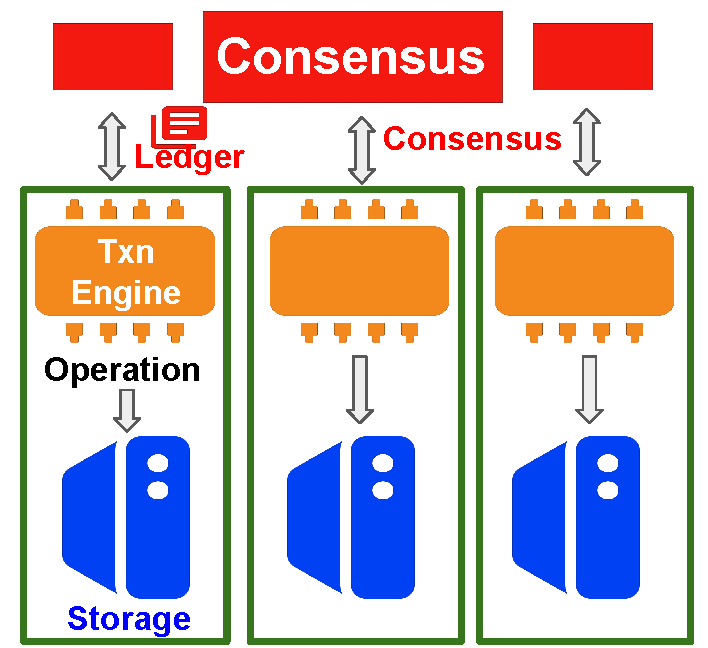
\includegraphics[width=0.99\textwidth]{diagram/twin/bc_arch.pdf}
	    % \caption{Blockchain architecture }
	    \caption{}
	\end{subfigure}%
	% \hspace{28mm}
	\begin{subfigure}{0.45\textwidth}
	    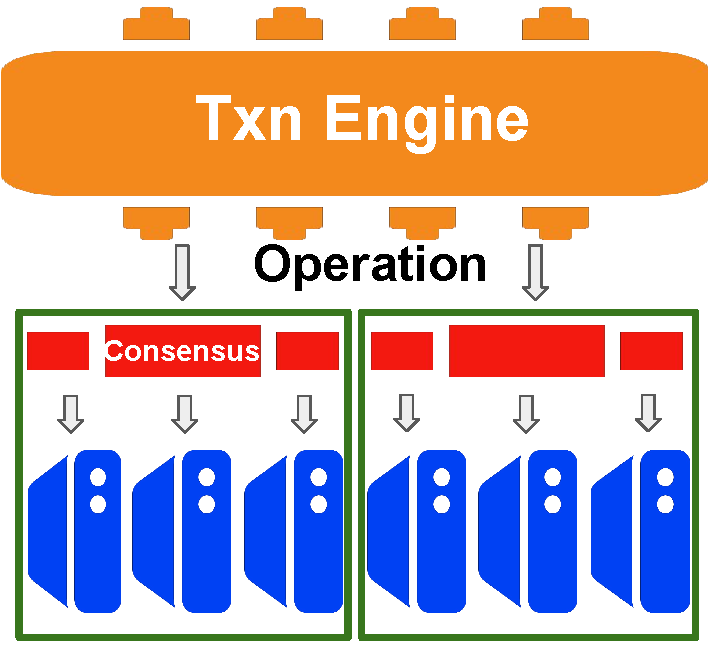
\includegraphics[width=0.99\textwidth]{diagram/twin/db_arch.pdf}
	    % \caption{Distributed database architecture}
	    \caption{}
    \end{subfigure}%
    \caption{Architecture of blockchains and distributed databases}
    \subcaption*{(a) Blockchains first reach consensus on the transaction history, then commit their effects into the storage.
    (b) Distributed databases replicate at the storage layer.}
    \label{diagram:twin:arch} 
\end{figure}

\subsubsection{Failure model}
Fault tolerance is an important goal of any distributed system. Distributed databases assume crash failure, in
which nodes only fail by crashing. In this model, referred to as crash fault tolerance (CFT), the system needs
to tolerate hardware and software crash, as well as network partition. CFT is suitable for databases, because
they are considered internal systems, protected by many layers of security. Blockchains, on the
other hand, assume hostile environments, in which a node can behave arbitrarily. In this Byzantine fault tolerance (BFT) model, the system needs to tolerate any software and hardware failures, as well as any malicious user. This model is appropriate when the system needs to operate correctly under security attacks. For example, the nodes may be compromised by an attacker and therefore deviate arbitrarily from the protocol. 

CFT protocols have lower security guarantees than BFT, but they can achieve higher performance for
a given number of failures. In particular, to tolerate $f$ failures, CFT requires $2f+1$ replicas, whereas BFT
requires $3f+1$. We observe that some permissioned blockchains support both failure models. For example,
Quorum provides both Raft~\cite{raft}, a CFT protocol, and Istanbul consensus, a BFT protocol,
implementation. These systems allow application developers to make different tradeoffs between security and performance. 


\subsubsection{Consensus protocol}
Permissionless blockchains adopt proof-of-work (PoW) or other variants such as proof-of-stake (PoS) and proof-of-elapsed time (PoE). In contrast, both permissioned blockchains and distributed databases adopt classic CFT or BFT protocols, such as Paxos~\cite{lamport2001paxos, lamport2006fast}, Raft~\cite{raft}, and PBFT~\cite{castro1999practical}. Detailed comparisons between PoW and other consensus protocols can be found in~\cite{dinh2018untangling,consensus_survey}. Here, we discuss the reason and implication of adopting PoW for permissionless blockchains. Our discussion also extends to other PoW variants.    

In the permissionless setting, a node or user can have many identities. The lack of strong identity
renders voting-based protocols --- most classic CFT and BFT protocols in the literature are voting-based ---
infeasible. PoW overcomes the identity problem by relying on incentives. In PoW, a node's probability of
solving a computational puzzle, thereby solving consensus and gaining rewards, is proportional to its
physical resources which are difficult to forge. Thus, the node has no advantage in having multiple
identities. 

In an asynchronous network, FLP theorem~\cite{fischer1982impossibility} rules out any deterministic
consensus protocol that can achieve both safety and liveness. Permissionless blockchains assume that nodes communicate
over the Internet which is subject to unpredictable performance and frequent partitioning. They opt for
liveness over safety, which means the system continues to work under network partitions, but these partitions may be in disagreement in the form of
chain forks, as shown in Figure~\ref{diagram:twin:fork}. For safety, permissionless blockchains rely on the network synchrony. In particular, when the partition time is longer than the block interval, nodes in each network partition independently append to the ledger. But when the network partition heals, transactions in shorter forks are discarded. This is the reason why permissionless blockchains require users to wait for transactions committed several blocks behind, before considering them in effect. We note that choosing liveness over safety is inevitable in the Internet environment because otherwise, the system will be unavailable for most of the time. 

\begin{figure}
    \centering
    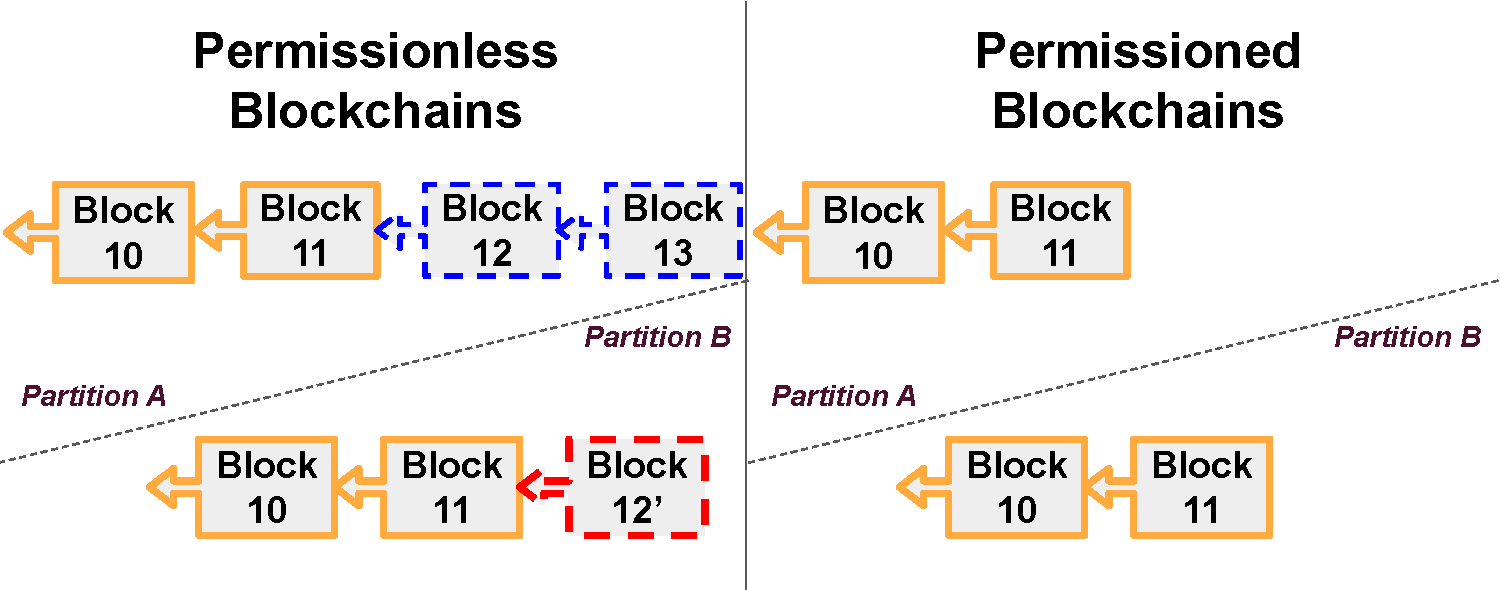
\includegraphics[width=0.9\textwidth]{diagram/twin/fork.pdf}
    \caption{Permissionless vs. permissioned blockchains during network partition after Block 11. The former keeps appending
    blocks in each partition, while the later becomes unavailable but remains consistent.} 
    \label{diagram:twin:fork} 
\end{figure}

PoW protocols are less sensitive to network conditions than classic CFT and BFT protocols because the latter are communication bound. In particular, most CFT and BFT incur $O(N)$ and $O(N^2)$ message complexity respectively, where $N$ is the network size. The delay of a single message may trigger the expensive recovery mode, which may worsen the delay and lead to performance collapse~\cite{dinh2017blockbench}. PoW protocols, on the other hand, are computation bound, in which the difficulty of the computational puzzle is adjusted gradually to approximate a fixed block interval. %%%
By not relying heavily on network communication, PoW blockchains achieve higher availability than permissioned blockchains and distributed databases.

\subsection{Concurrency}

Most blockchains execute transactions sequentially, while distributed databases employ sophisticated
concurrency control mechanisms to extract as much concurrency from the execution as possible. The reason for
blockchains' choice of serial execution is two-fold. First, serial execution may not affect the overall
performance because execution is often not the bottleneck. For example, in Bitcoin, the consensus protocol may
take several minutes, while transaction execution takes only a few seconds. Second, enforcing serial execution means the behavior of smart contracts
is deterministic when the transaction execution is replicated over many nodes. 
The benefit of determinism is that it is easy to reason about the states of the ledger, 
which simplifies the achievement of ACID equivalence in blockchains. 

Unlike blockchains, concurrency remains a major research topic in databases. To exploit more concurrency
inherent in the workloads, complex mechanisms are being proposed to ensure some forms of correctness. In
particular, there exists a wide range of isolation levels~\cite{computer1986american,bailis2013highly} which
make different tradeoffs between correctness and performance. Most production-grade databases today offer
more than one isolation level. 

We note that some blockchains start to employ parallelism and simple concurrency techniques used in databases. In Hyperledger Fabric,
for example, transactions are simulated (executed) in parallel against the ledger states before sent for ordering. During the later sequential commit, the
  system uses a simple optimistic concurrency control to achieve serializability which aborts
  transactions whose simulated states are stale. More established techniques to reduce abort have
  also been proposed~\cite{sharma2019blurring, ruan2020transactional}.

\subsection{Storage}
In this section, we describe how blockchains and distributed databases build different models and data
structures on the storage.  

\subsubsection{Storage model}
The storage in blockchains exposes an append-only ledger abstraction. The ledger records historical
transactions and the changes made to the global states. Some systems allow applications to access only
the latest states, for example, Hyperledger Fabric v0.6. Novel storage systems have been proposed to
enable access to any historical states during smart contract execution~\cite{ruan2019fine}. The storage in distributed databases, on the other hand, exposes direct access to data records. In databases without explicit provenance support, historical data is maintained in limited forms, for example as write-ahead logs.
We note that such logs are used primarily for failure recovery, and they are periodically pruned. 

\subsubsection{Index}
One of the most important properties of blockchains is data integrity, which means any tampering with the
data on the ledger must be detected. As a result, blockchains employ an authenticated data structure, such as Merkle tree index, to provide both efficient data access and integrity protection. For example, Ethereum uses a prefix trie, named Merkle
Patricia Trie (MPT)~\cite{web:mpt}. In the MPT, the states are stored at the leaves, and the ones with a common key
prefix are organized into the same branch. Each node is associated with the cryptographic hash of its
content, such that the root hash represents the complete global states. The access path serves as the
integrity proof for the retrieved value. Older versions of Hyperledger Fabric use a Merkle Bucket Tree (MBT)
in which the size of the tree is fixed. 

Indexes play such an instrumental role in databases that any small optimization on the index can translate
to significant improvement in performance. Modern indexes are designed to be hardware-conscious in order to
extract the most efficiency from the hardware. For example, in-memory databases abandon the disk-friendly B-tree
structure for other structures such as FAST~\cite{kim2010fast} and PSL~\cite{xie2017parallelizing} which
are designed for better cache utilization and multi-core parallelism.


\subsection{Sharding}

Sharding is a common technique in distributed databases for achieving scalability, in which data is
partitioned into multiple shards. Although it has been studied extensively
in databases, sharding has only recently been introduced to blockchains. In this section, we discuss two key
challenges in any sharded systems, that are (i) how to form a shard, and (ii) how to ensure atomicity for cross-shard
transactions.  

\subsubsection{Shard formation}
A shard formation protocol determines which nodes and data go to which shard. 
The security of blockchains depends on the assumption that the number of failures is below a certain
threshold. The shard formation protocol must, therefore, ensure that the assumption holds for every shard.  In
particular, the shard size must be large enough so that the fraction of Byzantine nodes is small.
Furthermore, the attacker must not be able to influence the shard assignment, otherwise, it could put enough
resources into one shard to break the security assumption. State-of-the-art sharded blockchains have different
approaches. For example, Elastico uses PoW for shard formation~\cite{luu2016secure},
OmniLedger~\cite{kokoris2018omniledger} employs a complex cryptographic protocol, while
AHL~\cite{dang2019towards} uses trusted hardware. The last two systems perform regular shard reconfiguration,
by re-executing the shard formation protocol, in order to guard against adaptive adversaries. 

The goal of sharding in distributed databases is scalability. As such, the systems aim to assign
data to shards in a way that optimizes the performance of certain workloads. In practice, they offer a variety of partitioning
schemes, for example, hash partitioning and range partitioning, so that users can select the most suitable
for their workloads.  Some systems, for instance, Cassandra\cite{lakshman2010cassandra}, even allow users to specify workload distributions so that data can be partitioned in a locality-aware manner. Unlike blockchains, shard reconfiguration is not necessary for databases, unless when there are significant changes in the workload distribution. 

\subsubsection{Atomicity}
Sharding introduces the problem of transaction atomicity when a transaction can touch data at multiple shards.
Atomicity requires the cross-shard transaction to either commit at all shards or not at all. In databases, this problem
is addressed by the two-phase commit (2PC) protocol. This protocol requires a dedicated transaction coordinator. This coordinator is trusted, but it may fail and leave
the transaction blocked forever. 
In a recent work, researchers propose Parallel Commit to reduce the commit path into a single round trip\cite{taft2020cockroachdb}. 

Sharded blockchains face additional challenges in ensuring atomicity because under the Byzantine failure
model the coordinator cannot be trusted. To overcome this, both~\cite{dang2019towards,herlihy2019cross} propose to implement a 2PC state machine in the shard that runs a BFT protocol. The BFT protocol ensures that the shard is less vulnerable to attacks and does not become a point of failure.
Any cross-shard transaction must involve this 2PC BFT replicated state machine to ensure atomicity. The consensus liveness guarantees the service high availability, therefore mitigating the blocking problem. 
But the Byzantine setup in blockchains imposes considerable overhead to the 2PC process.


\subsection{Fusion of Blockchains and Databases}
The taxonomy above  provides a comprehensive design space of distributed transactional systems, which helps
illustrate the similarities and differences between blockchains and distributed databases. It also serves as a principled framework for understanding the recently emerging hybrid blockchain-database systems. In this section, we compare these systems under our framework.

\textbf{Out-of-the-blockchain Databases.} One approach for hybrid design is to start with a blockchain and
build database features on top of it. Examples of this approach include BlockchainDB~\cite{el2019blockchaindb}, Veritas~\cite{veritas}, and
FalconDB~\cite{peng2020falcondb},  which provide shared and verifiable databases for multiple distrusting
parties.  They use blockchain only as an integrity-protected storage, and build other database components on
top of it. More specifically, BlockchainDB supports get/put/verify data operations.  FalconDB enables
verification from light-weight clients which do not have the full copy of the states. Veritas stores states in
a local database, and relies on voting and state digest in blockchains for disputes. In these
systems, replication is transaction-oblivious, with duplicated states, logs and meta-data.  Since
blockchain is on the critical path, these systems have limited performance.
BlockchainDB~\cite{el2019blockchaindb} employs multiple blockchains for storage, therefore it is amenable to
sharding.

\textbf{Out-of-the-database Blockchains.} Another approach for hybrid design is to start with a database,
then add blockchain features to it. Examples of this approach include
BigchainDB~\cite{mcconaghy2016bigchaindb}, Blockchain Relational Database (BRD)~\cite{BlockchainMeetsDatabase}
and ChainifyDB~\cite{schuhknecht2019chainifydb}. In these systems, each node has
its own stand-alone full-fudged database, and executes transactions on its database according to a global order achieved through
consensus. 
This is different from blockchains, such as Quorum, which embed LevelDB as a slim storage component and run it in the same process. 
In particular, BRD uses PostgreSQL and transactions contain invocation contexts of stored
procedures. BigchainDB uses MongoDB, thus its transactions are in JSON format.
ChainifyDB allows heterogeneous databases, and the nodes use consensus to agree on transaction effects instead
of transaction order. Both ChainifyDB and BRD use
Kafka broker service, a crash-tolerant consensus protocol that trades performance for security. In contrast,
BigchainDB uses Tendermint consensus protocol which tolerates Byzantine failures at the expense of performance.
In terms of concurrency, these systems inherit the concurrency support of their underlying databases, with
serializable constraints according to the ledger order.  However, these systems do not protect the local
states with Merkle trees, and only rely on the integrity protection of the ledger. 
Finally, these systems do not support sharding.

In summary, out-of-the-database blockchains retain many design choices of distributed databases, as their
main goal is performance. In contrast, out-of-the-blockchain databases inherit many design choices of
blockchains, as their main goal is security.

\section{Experimental Setup}
\label{twin:sec:setup}
\subsection{Systems}
We select five representative systems: two permissioned blockchains, namely Quorum~\cite{web:quorum} and Hyperledger Fabric~\cite{androulaki2018hyperledger}, two NewSQL distributed databases, namely CockroachDB~\cite{taft2020cockroachdb} and TiDB~\cite{huang13tidb}, and one NoSQL distributed database, namely Etcd~\cite{web:etcd}. 
Table~\ref{twin:tab:systems} summarizes their design choices according to the taxonomy in Section~\ref{twin:sec:anatomy}.

\begin{table*}[]
	\centering
	\caption{Comparison of the five selected systems based on our taxonomy}
	\label{twin:tab:systems}
	\resizebox{\textwidth}{!}{%
	\begin{tabular}{clcccccc}

		\toprule

		\multirow{2}{*}{System \& Version} & \multicolumn{3}{c}{\textbf{Replication}} & \multirow{2}{*}{\textbf{Concurrency}} & \multicolumn{2}{c}{\textbf{Storage}} & \multirow{2}{*}{\textbf{\begin{tabular}[c]{@{}c@{}}Sharding \\ Support\end{tabular}}} \\
		& \begin{tabular}[c]{@{}c@{}}Replication \\ Model\end{tabular} & \begin{tabular}[c]{@{}c@{}}Failure \\ Model\end{tabular} & \begin{tabular}[c]{@{}c@{}}Consensus \\ Protocol\end{tabular} &  & Storage Model & Index &  \\

		\midrule

		\multirow{2}{*}{\textbf{Quorum v1.8.2}} & \multirow{2}{*}{Transaction-based} & CFT & Raft & \multirow{2}{*}{Serial} & \multirow{2}{*}{Ledger-based} & \multirow{2}{*}{MPT} & \multirow{2}{*}{NO} \\
		&  & BFT & IstanbulBFT &  &  &  &  \\

		\multirow{2}{*}{\textbf{Fabric v2.2}} & \multirow{2}{*}{Transaction-based} & \multirow{2}{*}{CFT} & \multirow{2}{*}{Kafka} & Parallel Execution & \multirow{2}{*}{Ledger-based} & \multirow{2}{*}{LSM Tree} & \multirow{2}{*}{NO} \\
		&  & &  &  Serial Commit &  &  &  \\

		% \textbf{Hyperledger Fabric v1.3} & Transaction-based & CFT & Kafka & Parallel Execution Sequential Commit & Ledger-based & LSM Tree & NO \\
		\textbf{CockroachDB}\\ \textbf{v20.1.2} & Storage-based & CFT & Raft & Parallel & State-based & LSM Tree & YES \\
		\textbf{TiDB v2.1.0} & Storage-based & CFT & Raft & Parallel & State-based & LSM Tree & YES \\
		\textbf{Etcd v3.3.13} & Storage-based & CFT & Raft & Parallel & State-based & B-tree & NO \\

        \bottomrule
	\end{tabular}%
	}
\end{table*}

\textbf{Quorum}~\cite{web:quorum} (version $1.8.12$) is a permissioned blockchain based on Ethereum. It
targets the financial sector which requires greater efficiency and data privacy than what is provided by Ethereum.
Quorum replaces Ethereum's Proof of Work (PoW) with a CFT protocol, namely Raft, and a BFT protocol called
Istanbul BFT. However, it inherits the original Order-execute execution paradigm from Ethereum. \Cref{sec:literature:execution:order-execute} clarifies this architecture. 

\textbf{Fabric}~\cite{androulaki2018hyperledger} (version $2.2$) is a popular permissioned
blockchain started by IBM and the Linux Foundation. It has a modular design and features a novel execute-order-validate paradigm, as detailed in~\Cref{sec:literature:execution:execute-order-validate}. The system has two types
of nodes. 
{\em Peers} participate in the first execution and the last validation steps, simulating smart contracts, endorsing transactions and validating blocks. {\em Orderers} operate in the middle of the pipeline, reaching consensus on the transaction sequence and batch them into blocks. 

\textbf{CockroachDB}~\cite{taft2020cockroachdb} (version $20.1.2$) is 
a distributed NewSQL relational database that supports both ACID transactions and horizontal scalability. It relies on the Raft consensus protocol to synchronize replicas. As an open-source solution inspired by Spanner~\cite{corbett2013spanner}, CockroachDB utilizes a synchronized clock to coordinate Parallel Commit for transaction atomicity. 

\textbf{TiDB}~\cite{huang13tidb} (version $2.1.0$) is another distributed NewSQL database system that supports both SQL semantics and horizontal scalability. 
While CockroachDB takes a monolithic approach, TiDB is featured for its modular design. TiDB consists of three independent components, namely Placement Driver for coordinating cluster management, TiKV servicing as the replicated key-value storage, and TiDB-server for parsing and scheduling SQL queries in a stateless manner. 
TiDB also employs optimistic concurrency control and 2PC for transaction management, as well as Raft for replica consistency. However, its data isolation level only support snapshot isolation, more lenient than serializable in CockroachDB. 

\textbf{Etcd}~\cite{web:etcd} (version $3.3.13$) is a NoSQL database used in many large-scale
systems~\cite{web:etcd_user}.  
Etcd provides a simpler key-value data model with relaxed transactional restriction but focuses on the tradeoff between availability and consistency. 
Similar to blockchains, etcd employs a single consensus instance to sequence all the requests.
Without sharding, data are fully replicated on each node.

\subsection{Setup}
For a fair comparison, we run the five systems in full replication mode in which each node has a complete
copy of the states. In particular, for Fabric we use the endorsement policy under which a transaction
is executed and endorsed by all peers. For CockroachDB and TiDB, we set the replication factor to be the
same as the number of nodes. 

We use CFT protocols in all five systems. In particular, we configure Quorum to use Raft, and Fabric to use
Kafka which is a CFT protocol. We also disable all optional security features, such as data encryption and
Transport Layer Security (TLS) communication. 

We set the number of transactions per block to $100$ in Fabric and the block interval to the
minimum in Quorum. We scale all TiDB's modules with the number of nodes so that each node runs all three
modules in different processes. For Fabric, we run the orderers on two nodes and Kafka on three nodes.

Unless otherwise specified, we use the YCSB and Smallbank workloads in our experiments. The experiment
parameters for YCSB are summarized in Table~\ref{twin:tab:parameter} with the default values underlined. 
All the experiments are repeated three times and we report the average .

\begin{table}
	\centering
	\caption{Experiments parameters in YCSB workload to benchmark blockchains and distributed databases. }
	\label{twin:tab:parameter}
	\begin{tabular}{@{}ll@{}}
	\toprule
	\textbf{Variable}               & \textbf{Values}               \\
	\midrule
	Record size (Byte)               & 10, 100, \underline{1000}, 5000          \\
	Zipfian coefficient $\theta$       & \underline{0.0}, 0.2, 0.4, 0.6, 0.8, 1.0 \\
	\# of transaction operations & \underline{1}, 2, 4, 6, 8, 10            \\
	\# of nodes & 3, \underline{5}, 7, 11, 15, 19            \\
	\bottomrule
	\end{tabular}
\end{table}


\subsection{Benchmark Driver}
We note that existing benchmark drivers for databases are synchronous (or closed-loop), meaning that a next
request is sent only after the current request is completed. In contrast, blockchain benchmark
drivers, such as Fabric's Caliper and BLOCKBENCH driver~\cite{dinh2017blockbench}, are asynchronous (or
open-loop) in which a new request is sent as soon as the current request is acknowledged by a
node in the blockchain. 
Figure~\ref{diagram:twin:driver_diff} illustrates the difference between the two types of drivers. 
In a synchronous driver, a separate status thread is responsible for computing statistics. In an
asynchronous driver, the status thread needs to keep track of outstanding requests and to periodically poll
the blockchain for newly completed requests. 

Asynchronous drivers are suitable for blockchains because of the long request latency which requires a large number of outstanding requests to saturate the system. In other words, benchmarking a blockchain with synchronous drivers would require many nodes to run the driver. 
To verify this, we implement a synchronous YCSB driver for Fabric using its Java SDK.  
Our results show that its measured peak throughput is capped around 20 tps, while Caliper reports 400 tps. 
In other words, the synchronous driver severely underestimates Fabric's performance, even with a large number of client-side requests issued.

\begin{figure}
    \centering
    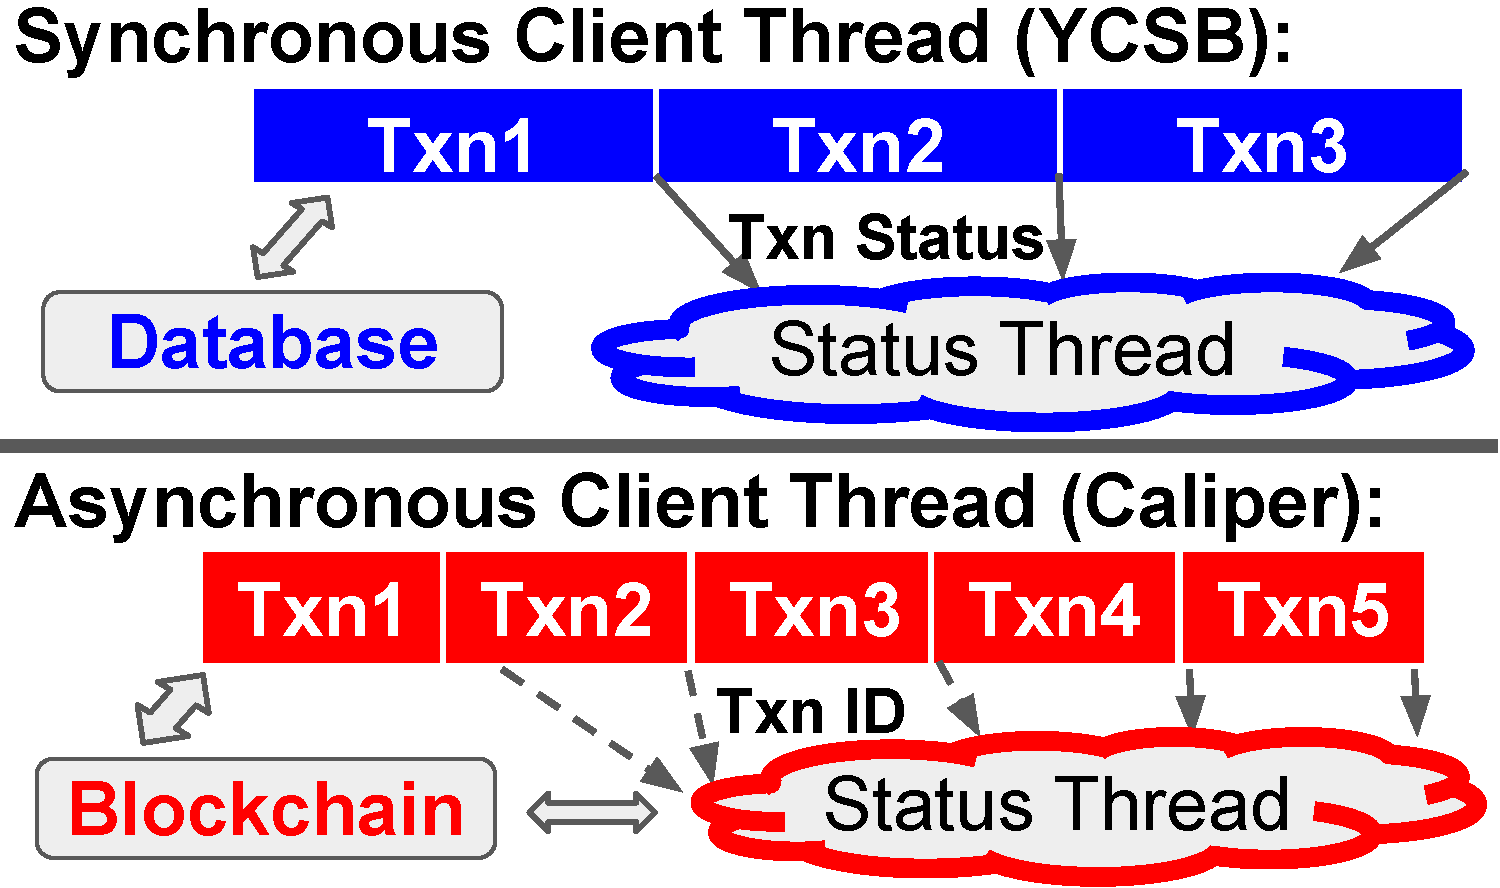
\includegraphics[width=0.7\textwidth]{diagram/twin/driver_diff.pdf}
    \caption{Differences between synchronous and asynchronous drivers.}
    \subcaption*{Asynchronous drivers can issue more transactions, as they do not have to wait for their completion, as opposed to the synchronous ones.}
    \label{diagram:twin:driver_diff} 
\end{figure}

For the database experiments we use the open-source driver for YCSB workload~\cite{web:ycsb} and 
the OLTPBench~\cite{difallah2013oltp} driver for Smallbank workload.  Both Fabric and Quorum are
benchmarked using Caliper~\cite{web:caliper}. We note that although there are differences in the types of
drivers for benchmarking blockchains and databases, they alone do not account for the large performance gap
reported in the following section. 

\section{Performance Analysis}
\label{twin:sec:result}
We start by summarizing our main experimental findings and continue with the detailed analysis.
\begin{itemize}
  \item \textbf{Peak performance. }  The performance gap between blockchains and distributed databases is large. However, the gap is not as significant as previously reported. 
  \item \textbf{Replication. } The single-instance replication in blockchains hinders their horizontal 
  scalability. The performance of systems with BFT consensus is more sensitive to network conditions compared to systems with  
  CFT consensus. 
  \item \textbf{Concurrency. } Both databases and blockchains that adopt the execute-order-validate execution 
  model have low performance under workloads with high contention and constraints.  On the other hand, their
  performance is not impacted by long-lasting transactions, unlike blockchains with the order-execute model.
  \item \textbf{Storage. } The ledger abstraction in blockchains incurs significant storage overhead. On the 
  other hand, the overhead needed to guarantee state tamper evidence is small.
  \item \textbf{Sharding. } The performance of sharded blockchains is far behind that of distributed
  databases, due to the security requirements on shard formation and periodic reconfiguration.
\end{itemize}